\documentclass[12pt,a4paper]{article}

\usepackage[brazil]{babel}
\usepackage[utf8]{inputenc}
\usepackage[T1]{fontenc}
\usepackage{graphicx}
\usepackage{epsfig}
\usepackage{cite}
\usepackage{verbatim}
\usepackage{concrete}
\usepackage{amsfonts}
\usepackage{amsmath}
\usepackage{amssymb}
\usepackage{setspace}
\usepackage{url}
\usepackage{subfigure}
\usepackage{array}
\usepackage{multirow}
\usepackage{colortbl}
\usepackage{tabularx}
\usepackage{geometry}
\usepackage{cite}
\usepackage{xcolor}
\usepackage{color}
\usepackage{url}
\usepackage{lmodern}
\usepackage{pict2e}
\usepackage{siunitx}

\geometry{top=2.3cm,bottom=2.2cm,left=2.5cm,right=2.5cm}

\newcommand{\V}[1]{\boldsymbol{#1}}

\providecommand{\todo}[1]{{\textbf{\protect\color{red} {TODO: #1}}}}

\newenvironment{myitemize}{
\begin{itemize}
 \setlength{\itemsep}{1pt}
 \setlength{\parskip}{0pt}
 \setlength{\parsep}{0pt}
}{\end{itemize}}

\newenvironment{myenumerate}{
\begin{enumerate}
 \setlength{\itemsep}{1pt}
 \setlength{\parskip}{0pt}
 \setlength{\parsep}{0pt}
}{\end{enumerate}}

%  ABACO -- Conjunto de macros para desenhar o 'abaco

%  Desenho original de Hans Liesenberg

%  Macros de Tomasz Kowaltowski

%  DCC -- IMECC -- UNICAMP

%  Mar,co de 1988  --  Vers~ao 1.0

% Ajustado para LaTeX da SUN -- Mar,co de 1991

% ---------------------------------------------------------

%  Chamada:   \ABACO{d1}{d2}{d3}{d4}{esc}
%             com:  di's -- os quatro d'igitos;
%	           esc  -- fator de escala

% ---------------------------------------------------------

%  DEFINI,C~OES AUXILIARES

% ---------------------------------------------------------


%  Forma o d'igito pequeno (0 ou 1)

\newcommand{\ABACODP}[1]{%
%
\thicklines
%    
\begin{picture}(8,0)
    \ifcase#1{   %  caso 0
       \put(0,0)    {\line(1,0){4}}
       \multiput(5,0)(2,0){2}{\oval(2,4)}}
    \or{         %  caso 1
       \put(2,0)    {\line(1,0){4}}
       \multiput(1,0)(6,0){2}{\oval(2,4)}}
    \fi
\end{picture}
    } % \ABACODP

% Forma o d'igito grande (0 a 4)

\newcommand{\ABACODG}[1]{%
%
\thicklines
%    
\begin{picture}(14,0)
    \ifcase#1{   % caso 0
       \multiput(1,0)(2,0){5}{\oval(2,4)}}
       \put(10,0)   {\line(1,0){4}}
    \or{         % caso 1
       \multiput(1,0)(2,0){4}{\oval(2,4)}}
       \put(8,0)   {\line(1,0){4}}
       \put(13,0)   {\oval(2,4)}
    \or{         % caso 2
       \multiput(1,0)(2,0){3}{\oval(2,4)}
       \put(6,0)   {\line(1,0){4}}
       \multiput(11,0)(2,0){2}{\oval(2,4)}}
    \or{         % caso 3
       \multiput(1,0)(2,0){2}{\oval(2,4)}
       \put(4,0)   {\line(1,0){4}}
       \multiput(9,0)(2,0){3}{\oval(2,4)}}
    \or{         % caso 4
       \put(1,0)  {\oval(2,4)}}
       \put(2,0)   {\line(1,0){4}}
       \multiput(7,0)(2,0){4}{\oval(2,4)}
    \fi
\end{picture}
    } % \ABACODG
       
% Forma um d'igito (0 a 9)

\newcommand{\ABACOD}[1]{%
%
    \ifnum#1>9
       \errmessage{#1: Argumento invalido para ABACO}
    \fi
    \ifnum#1<0
       \errmessage{#1: Argumento invalido para ABACO}
    \fi
%
\begin{picture}(24,0)
%    
    \ifnum#1<5
       \put(16,0) {\ABACODP{0}}
    \else   
       \put(16,0) {\ABACODP{1}}
    \fi
%    
    \ifnum#1<5
       \put(0,0)  {\ABACODG{#1}}
    \else
       \ifcase#1\or \or \or \or
          \or  \put(0,0)  {\ABACODG{0}}
          \or  \put(0,0)  {\ABACODG{1}}
          \or  \put(0,0)  {\ABACODG{2}}
          \or  \put(0,0)  {\ABACODG{3}}
          \or  \put(0,0)  {\ABACODG{4}}
       \fi
    \fi   
\end{picture}
    } % \ABACOD
    
% -------------------------------------------------

%  DEFINI,C~AO PRINCIPAL
    
\newcommand{\ABACO}[5]{%
    \setlength{\unitlength}{#5mm}
%
    \thinlines
%   
\begin{picture}(28,25)
%   
% moldura
%
% externa
%
        \put(0,0)            {\line(0,1){25}}
        \put(0,0)            {\line(1,0){28}}
        \put(28,0)           {\line(0,1){25}}
        \put(0,25)           {\line(1,0){28}}
% interna
        \put(2,2)            {\line(0,1){21}}
	\put(26,2)           {\line(0,1){21}}
	\put(16,2)           {\line(0,1){21}}
	\put(18,2)           {\line(0,1){21}}
	\put(2,2)            {\line(1,0){14}}
	\put(16,2)           {\line(1,-1){1}}
	\put(17,1)           {\line(1,1){1}}
	\put(18,2)           {\line(1,0){8}}
	\put(2,23)           {\line(1,0){14}}
	\put(16,23)          {\line(1,1){1}}
	\put(17,24)          {\line(1,-1){1}}
	\put(18,23)          {\line(1,0){8}}
	\put(0,0)            {\line(1,1){2}}
	\put(0,25)           {\line(1,-1){2}}
	\put(28,0)           {\line(-1,1){2}}
	\put(28,25)          {\line(-1,-1){2}}
%
%   
% d'igitos
%
%   
       \put(2,20)  {\ABACOD{#1}}
       \put(2,15)  {\ABACOD{#2}}
       \put(2,10)  {\ABACOD{#3}}
       \put(2,5)   {\ABACOD{#4}}
%      
\end{picture}
    } % \ABACO
    


\begin{document}

\tolerance = 999
\sloppy

\hyphenation{re-co-nhe-ci-men-to}
\hyphenation{ca-rac-te-rís-ti-cas}
\hyphenation{a-pre-sen-ta-ção}
\hyphenation{pos-si-bi-li-ta-rá}

\thispagestyle{empty}

\begin{center}{\large \bf UNIVERSIDADE ESTADUAL DE CAMPINAS} \end{center}
\begin{center}{\large INSTITUTO DE COMPUTAÇÃO} \end{center}

\begin{center}
\begin{minipage}[tl]{31mm}
  \ABACO{1}{9}{6}{9}{1}
\end{minipage}
\end{center}

\vspace*{3.5cm}

\begin{center}
{\Large \bf MC833 - Relatório Científico 1}

\vspace*{2.0cm}

\textsc{\Large Comunicação Cliente-Servidor} \\ [0.1cm]
\textsc{\Large Usando Protocolo UDP}

\vspace{2.5cm}

\textbf{135368:} Cristina Freitas Bazzano \\
\textbf{135749:} Flávio Altinier Maximiano da Silva

\vspace{7.5cm}

{\large Campinas - SP}
\vspace*{0.2cm}

{\large Abril de 2015}
\end{center}

\clearpage

\pagenumbering{arabic}
\onehalfspacing
\tableofcontents 
\clearpage
\onehalfspacing

\begin{abstract}
Este trabalho focou-se no estudo temporal de redes cliente-servidor baseadas em comunicação UDP e um comparativo com um estudo anterior baseado em comunicação TCP. Foi implementado um serviço de locadora de filmes baseado em {\it MySQL} no servidor, e ao cliente foram adicionadas diversas operações de acesso ao banco, baseando-se em operações de consultas pequenas, grandes e de escrita. Observou-se que a escrita no banco é o processo mais lento, enquanto operações de consultas extensas são apenas brevemente mais lentas que buscas mais curtas, o que também ocorreu com o TCP. Outro ponto interessante medido foi a confiabilidade das transmissões, em ambos os protocolos nenhuma mensagem foi perdida. Notamos também que o tempo total de comunicação no protocolo UDP foi cerca de 10 vezes menor que o TCP. Além disso, uma breve análise de tamanho de código mostrou que operações de redes não são as mais presentes em uma implementação desse tipo.
\end{abstract}

\section{Introdução}
Na Internet, a grande maioria das montagens de comunicação baseia-se em um sistema cliente-servidor. Nesse contexto, o servidor guarda alguma informação que é relevante ao cliente, que pede essa informação através de uma mensagem na rede; o servidor, por sua vez, responde esse pedido com outra(s) mensagem(ns) contendo a informação requisitada.

O protocolo da camada de transporte escolhido para este projeto é o {\it User Datagram Protocol} (UDP)~\cite{postel1980user}. Tal protocolo não garante confiabilidade: é baseado em troca rápida de mensagens, e sem {\it hand shaking}. Neste trabalho faremos uma comparação com um trabalho anterior que realizou as análises usando o protocolo {\it Transmission Control Protocol} (TCP)~\cite{postel1981transmission}, que por outro lado é confiável.

Neste trabalho, num primeiro momento, o foco principal de nossa análise será a medida de tempo total de comunicação entre cliente e servidor, além de uma aproximação do tempo de transmissão das mensagens entre os dois (tempo de as mensagens saírem de um host e chegarem ao outro). Analisaremos também brevemente a confiabilidade das mensagens enviadas, que não é garantida pelo protocolo. Em seguida faremos uma comparação desses resultados com aqueles obtidos em um trabalho passado que analisou o protocolo TCP. O tamanho do código será também analisado, além de um breve parecer sobre o nível de abstração do sistema desenvolvido.

\section{Descrição Geral do Sistema}

O sistema construído consiste em uma simples montagem de cliente-servidor, com comunicação UDP. Como discutido, tal protocolo não garante que as mensagens enviadas efetivamente chegarão ao destinatário, nem que chegarão na ordem correta.

    O sistema montado é uma emulação de um serviço de locadora online, onde o servidor contém diversas informação sobre os filmes que possui em seu estoque, os quais podem ser acessadas por clientes ou pelo cliente administrador da locadora. 
    
    Para sintetizar o problema da melhor forma possível, criamos no nosso banco de dados uma tabela “Locadora” que armazena os seguintes atributos sobre os filmes que possui: título, ano de lançamento, gênero, duração, sinopse, diretor, ator principal, ator coadjuvante principal, exemplares e um id único para cada filme. 
    
Os acessos do cliente ou do administrador do locadora ao servidor são com pedidos de informação ou escrita de dados de cada filme, sendo eles da seguinte forma:

\begin {myenumerate}
\item Listar todos os títulos dos filmes e o ano de lançamento;
\item Listar todos os títulos dos filmes e o ano de lançamento de um gênero determinado;
\item Dado o identificador de um filme, retornar a sinopse do filme;
\item Dado o identificador de um filme, retornar todas as informações deste filme;
\item Listar todas as informações de todos os filmes;
\item Alterar o número de exemplares em estoque;
\item Dado o identificador de um filme, retornar o número de exemplares
em estoque.
\end{myenumerate}

    Todos esses acessos podem ser feitos em dois modos de consulta: um que realiza a consulta apenas uma vez, para testar sua corretude, e outro que realiza a consulta sequencialmente; cada acesso é repetido 30 vezes e todos os tempos são armazenados em um arquivo {\it log}, para possibilitar uma futura análise dos mesmos.
    
    Classificamos esses acessos em 3 categorias: as consultas pequenas, consultas grandes e operações de escrita. De acordo com a consulta que cada operação realiza podemos dividi-las da seguinte forma: no primeiro grupo se encontram as operações de 1 a 4 e a operação 7, no segundo grupo temos apenas a operação 5 e no terceiro grupo temos a operação 6. 
    
O primeiro grupo é caracterizado por uma consulta rápida de até 1500 bytes, que é o tamanho máximo MTU (Maximum Transmission Unit) que um pacote pode ter para ser transmitido pela camada Ethernet. O segundo grupo realiza consultas longas, com mais de 1500 bytes, que devem ser quebradas em mais de um pacote para serem enviadas. E o terceiro grupo é caracterizado por uma consulta que carrega um maior atraso do bando de dados, uma vez que no tempo medido está embutido o tempo de escrita no banco.


\section{Armazenamento e Estruturas de Dados}

Em um sistema real de cliente-servidor os dados são em sua maioria armazenados em Banco de Dados para garantir a persistência e a consistência dos mesmos. Com o objetivo de nos aproximar o máximo possível de um problema real, adotamos o MySQL~\cite{mysql1995mysql} como o Banco de Dados para armazenar os dados da locadora de filmes no servidor.

    Populamos o banco do servidor com dados de 10 filmes retirados do site IMDb~\cite{IMDbsite}, os quais estão classificados com as 10 melhores notas no mesmo. Optamos por uma quantia pequena de exemplares para que os tempos medidos nas operações não fossem totalmente influenciados pelo tempo de acesso ao servidor, visto que os tempos de comunicação são o foco da análise do projeto.
    
    No acesso ao banco de dados, os clientes podem apenas acessar a informação, enquanto o cliente administrador da locadora pode, além do acesso, alterar a quantidade de exemplares em estoque. Para garantir esse privilégio de acesso, é necessário uma senha para entrar no modo administrador, a qual é processada pelo programa e só após confirmada o acesso diferenciado ao banco pode ocorrer.
    
Com o objetivo de fazer um sistema robusto, o lado do Cliente na aplicação desenvolvida também tem uma cópia do banco de dados. Esse banco local serve para verificar os resultados do servidor remoto: se a resposta do servidor for diferente da esperada (que já é conhecida devido ao banco de dados local), essa diferença também é salva pelo experimento.

\section{Detalhes de Implementação}

Tanto o cliente quanto a servidor foram implementados baseando-se nas descrições encontradas em~\cite{hall19beej}. A porta do servidor escolhida para comunicação foi a porta “35368”.

Para o servidor, o socket de “escuta” é iniciado com o auxílio da operação {\it getaddrinfo()}; o tipo de socket é o SOCK\_DGRAM, que caracteriza uma comunicação UDP.

O servidor entra em um loop no qual fica aceitando mensagens na ordem em que chegam, com a função {\it recvfrom}(). Ao receber a mensagem, a processa e envia a resposta com {\it sendto}(), para o mesmo cliente recebido pela chamada a {\it recvfrom}().

No cliente, seguimos a comunicação também como descrito~\cite{hall19beej}: o socket de comunicação também é criado com o auxílio de {\it getaddrinfo()}. Em ambos os casos, como a comunicação é feita em LAN, a função retorna apenas as informações de cliente e servidor diretamente, então não é necessário o loop como feito na literatura~\cite{hall19beej}. Como estamos trabalhando com apenas um servidor, no lado do cliente podemos usar a função {\it connect}() como se fosse comunicação TCP. O conceito é diferente, entretanto: enquanto no protocolo TCP o {\it connect}() enviava a mensagem de {\it hand-shaking} ao servidor, no UDP ela apenas salva localmente o destino e remetente de {\it send}() e {\it recv}(), respectivamente.

A função {\it recv}() do cliente, entretanto, é levemente diferente: como no UDP mensagens podem se perder, pode ser que a requisição ao servidor, ou sua resposta ao cliente, se percam na rede. Dessa forma, o cliente ficaria bloqueado esperando uma resposta para sempre. Usamos então em nossa vantagem a função {\it select}(), que nos permite usar um limite de tempo para esperar a resposta. Colocamos esse tempo como $\SI{3.5}{\second}$: se a resposta do servidor demorar mais que isso, consideramos que ela se perdeu na rede e partimos para a próxima requisição.

O cliente, a cada vez que é iniciado, joga na tela um {\it prompt} com as opções de requisição ao servidor. Em seguida, após escolhida a opção, o cliente dá a opção de fazer o acesso apenas uma vez (para verificar a corretude da aplicação) ou trinta vezes. Se o usuário escolher por fazer o acesso apenas uma vez, o resultado da consulta é exibido na tela do cliente. Se escolher por fazer a consulta trinta vezes, um arquivo de {\it log} de respostas é criado na mesma pasta do cliente, com o nome {\it testX.txt}, onde {\it X} é o número do teste escolhido pelo usuário no {\it prompt}.

A consulta é feita ao servidor pelo meio de envio de consultas {\it MySQL}, que são montadas no próprio programa do cliente. Essas consultas são enviadas como mensagens ao servidor que simplesmente as aplica ao seu banco de dados e retorna o resultado das consultas de leitura ou escrita, também em forma de mensagens. Essa mesma consulta é aplicada a um banco de dados local no cliente, que é exatamente igual ao do servidor; o resultado local dessa consulta é usado para verificar a confiabilidade do resultado enviado pelo servidor.

Esse arquivo de {\it log} gerado tem o seguinte formato: são trinta linhas e duas colunas, onde cada linha representa um dos testes. A primeira coluna representa o tempo total de comunicação entre cliente e servidor (desde imediatamente antes do {\it send}() até imediatamente depois do {\it recv}()); a segunda coluna traz um valor numérico da seguinte forma: se a mensagem recebida for igual à gerada no banco de dados local, ou seja, se a transmissão foi confiável e as mensagens chegaram corretamente, esse valor é zero. Qualquer outro valor diferente de zero significa que houve corrupção de mensagens. 

O servidor também concatena a um arquivo de {\it log} dados sobre cada conexão que coordena. Como o servidor concatena informações num mesmo arquivo, quando o cliente fizer, por exemplo, trinta consultas de títulos de filmes, as últimas trinta entradas desse {\it log} do servidor guardarão os dados sobre essas consultas. Cada entrada nesse {\it log} é um {\it float} que guarda o tempo de acesso do servidor ao banco de dados; esse tempo é o intervalo desde imediatamente após o {\it recvfrom()} da consulta até imediatamente antes do {\it sendto()} do resultado. Dessa forma, podemos calcular o tempo de transmissão das mensagens: usando o tempo $ tServer $ desse {\it log} do servidor e a segunda coluna do {\it log} do cliente ($ tClient $), o tempo de transmissão de uma mensagem ao outro será dado por:
\begin{equation}
{\text {Tempo de Transmissão}} = \frac{tClient - tServer}{2}
\label{eqn:time}
\end{equation}
Um outro pequeno detalhe de implementação é que apenas o cliente administrador da locadora deve ter autorização para alterar o número de exemplares em estoque de cada filme. Portanto, quando um cliente decide fazer essa alteração, é perguntado por uma senha. Essa senha é verificada no próprio programa do cliente (é hard-coded como “1234”) e, apenas se estiver correta, o programa continua. Essa escrita no banco de dados também é hard-coded para garantir a consistência entre o banco de dados local e o remoto (do servidor), para que posteriormente possa ser verificada a confiabilidade das mensagens. Numa situação de mundo real, onde não há banco de dados local, essa opção não pode ser hard-coded.

O tamanho máximo de buffer adotado é de um milhão de caracteres; o tamanho máximo das consultas são 150 caracteres.


\section{Análise dos Resultados}

Toda a comunicação foi feita em LAN, com cliente e servidor conectados a um roteador D-Link DIR-600 por Wi-fi.

\subsection{Tempo total de Comunicação}

Em todos os resultados dos tempos médios utilizamos um intervalo de confiança com nível de confiança de 95\%, obtido a partir da soma ou subtração de dois desvios padrão.

Temos nesta seção temos os resultados dos experimentos usando o protocolo UDP; temos também os resultados para os mesmos experimentos usando TCP, de um relatório feito anteriormente, e esses dados serão comparados.
    
Primeiramente geramos um gráfico com o tempo total de conexão com o servidor para cada uma das operações. O resultado segue demonstrado na Tabela~\ref{table:totalU} e na Figura~\ref{fig:totalU}.

\begin{table}[h]
\centering
\caption{Tabela mostrando o tempo médio e intervalo de confiança para cada uma das sete operações, na ordem em que foram descritas, para o protocolo UDP. Tempo calculado no cliente, desde o envio da mensagem até o recebimento da resposta.}
\label{table:totalU}
\begin{tabular}{lll}
Operação & Tempo Médio Total (\SI{}{\milli\second})  & Intervalo de Confiança (\SI{}{\milli\second})           \\
1        & 2.52 & 3.47  \\
2        & 2.85 & 8.02 \\
3        & 2.76 & 6.67 \\
4        & 2.89 & 6.44 \\
5        & 7.31 & 4.27 \\
6        & 53.83 & 15.95 \\
7        & 3.07 & 7.23
\end{tabular}
\end{table}

Observe também na Tabela~\ref{table:totalT} e na Figura~\ref{fig:totalT} os resultados de tempo total de conexão, desde o {\it connect}() até o {\it close}(), para o protocolo TCP, para os mesmos experimentos.

\begin{figure}[h]
\centering
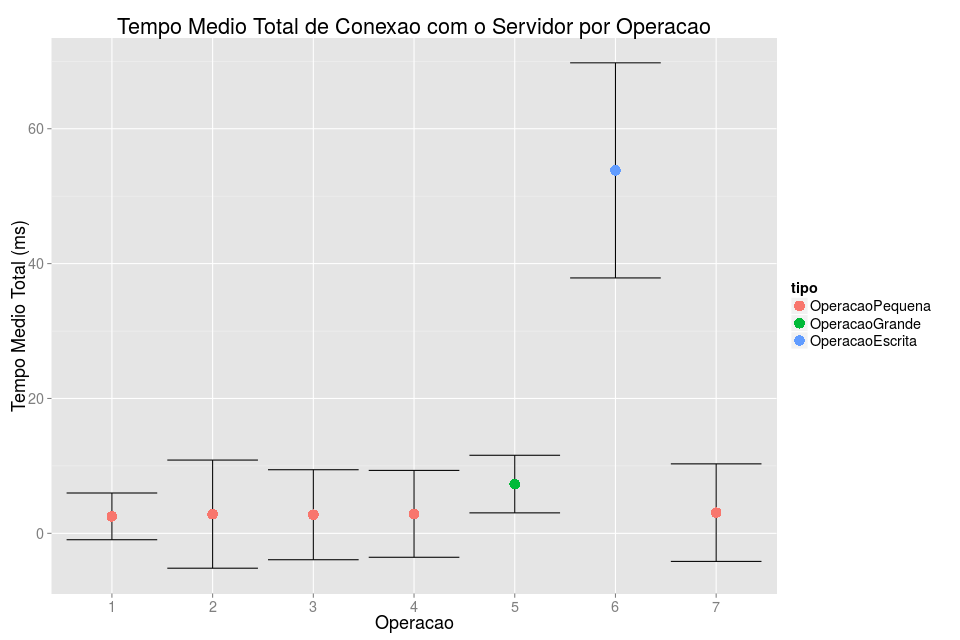
\includegraphics[width=\textwidth]{diagrama/resultadosTempoTotalUDP.png}
\caption{Mostra o tempo médio e o intervalo de confiança de 95\% para as sete operações, na mesma ordem em que foram descritas, utilizando-se o protocolo UDP. Tempo calculado no cliente, o envio da mensagem ao servidor, até a recepção da resposta.}
\label{fig:totalU}
\end{figure}

\begin{table}[h]
\centering
\caption{Tabela mostrando o tempo médio e intervalo de confiança para cada uma das sete operações, na ordem em que foram descritas, para o protocolo TCP. Tempo calculado no cliente, desde a abertura até o fechamento da conexão.}
\label{table:totalT}
\begin{tabular}{lll}
Operação & Tempo Médio Total (\SI{}{\milli\second}) & Intervalo de Confiança (\SI{}{\milli\second})\\ \hline
1        & 38.42           & 5.59   \\
2        & 37.38           & 9.14   \\
3        & 37.47           & 7.59   \\
4        & 37.10           & 10.37  \\
5        & 40.41           & 9.15   \\
6        & 114.10          & 95.27  \\
7        & 36.49           & 7.88  
\end{tabular}
\end{table}

\begin{figure}[h]
\centering
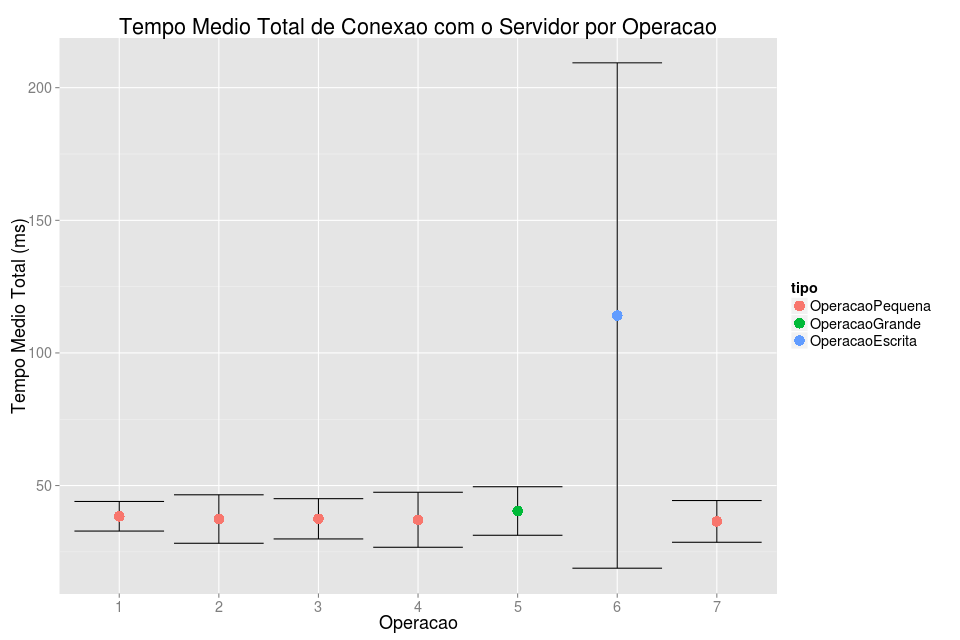
\includegraphics[width=\textwidth]{diagrama/resultadosTempoTotal.png}
\caption{Mostra o tempo médio e o intervalo de confiança de 95\% para as sete operações, na mesma ordem em que foram descritas, para o protocolo TCP. Tempo calculado no cliente, desde a abertura até o fechamento da conexão.}
\label{fig:totalT}
\end{figure}

Os resultados que obtivemos para o tempo total de conexão dependem bastante das consultas ao banco de dados e do tamanho das mensagens. Essas mensagens nas operações pequenas, como já especificado, podem ser totalmente enviadas em apenas um pacote, enquanto nas operações grandes, vários pacotes são necessários para o envio completo das mensagens. Nas operações de escrita, apesar de só um pacote ser necessário para o envio da mensagem, a consulta ao banco de dados para alteração requer um tempo bem maior de operação.

Com isso em mente, os resultados foram como esperado. Observe que tanto no TCP quanto no UDP as operações de escrita notoriamente tomam mais tempo que as outras. É notável também que as operações grandes levam um pouco mais de tempo que as pequenas - mas ainda têm tempos bem inferiores às de escrita.

O fato a se notar, entretanto, é a escala vertical dos gráficos: embora eles sejam parecidos, em todas as operações o TCP tomou mais tempo que o UDP. Em todos os experimentos realizados, essa afirmação mostrou-se verdadeira.

\subsection{Tempo de Transmissão}

Em seguida geramos um gráfico com o tempo total de transmissão das mensagens para cada uma das operações, como explicitado pela equação~\ref{eqn:time}. O resultado para o UDP segue na Tabela~\ref{table:transmissaoU} e Figura~\ref{fig:transmissaoU}. Na Tabela~\ref{table:transmissao} e Figura~\ref{fig:transmissao} temos os resultados para os mesmos experimentos utilizando o protocolo TCP.

\begin{table}[h]
\centering
\caption{Mostra o tempo médio e intervalo de confiança de 95\% para transmissão de mensagens segundo a equação~\ref{eqn:time} para cada uma das operações, na ordem em que foram descritas, utilizando o protocolo UDP.}
\label{table:transmissaoU}
\begin{tabular}{lll}
Operação & Tempo Médio de Transmissão (\SI{}{\milli\second}) & Intervalo de Confiança (\SI{}{\milli\second}) \\ \hline
1        & 1.14           & 1.71 \\
2        & 1.32 & 3.99 \\
3        & 1.28 & 3.33 \\
4        & 1.34         & 3.22 \\
5        & 3.13 & 2.06 \\
6        & 1.37 & 1.16 \\
7        & 1.43           & 3.61 
\end{tabular}
\end{table}

Os tempos de transmissão medem o tempo de comunicação entre o cliente e o servidor. Esse tempo deve depender apenas do tamanho das mensagens, que como já especificado, corresponde apenas a um pacote nas operações pequenas e de escrita e de vários pacotes nas operações grandes. 

Os tempo obtidos para as operações pequenas e grandes condizem com essa expectativa, tanto no TCP quanto no UDP; no TCP, entretanto, as operações de escrita em alguns experimentos tiveram tempos de transmissão muito maiores (observe o alto desvio): acreditamos que isso se deva às aproximações no cálculo do tempo de transmissão. Para o UDP, entretanto, o tempo de transmissão foi totalmente dentro do esperado: operações pequenas e de escrita levaram quase sempre o mesmo tempo; operações grandes precisaram de um intervalo de tempo maior para serem transmitidas.

Note que os tempos de transmissão das mensagens UDP foram muito inferiores aos tempos do TCP;  enquanto uma operação grande demorou cerca de $\SI{10}{\milli\second}$, em média, para ser transmitida no TCP, no UDP levou apenas $\SI{3}{\milli\second}$, em média.

\begin{figure}[h]
\centering
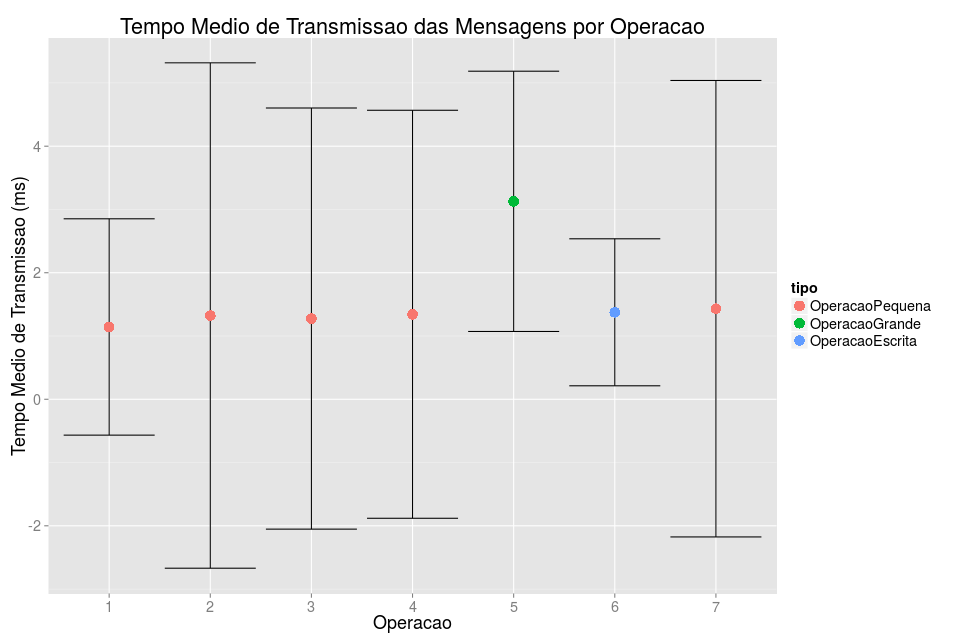
\includegraphics[width=\textwidth]{diagrama/resultadosTempoTransmissaoUDP.png}
\caption{Tempo médio, com intervalo de confiança de 95\%, calculado conforme a equação~\ref{eqn:time}, para as sete operações na mesma ordem em que foram descritas, utilizando o protocolo UDP.}
\label{fig:transmissaoU}
\end{figure}

\begin{table}[h]
\centering
\caption{Mostra o tempo médio e intervalo de confiança de 95\% para transmissão de mensagens segundo a equação~\ref{eqn:time} para cada uma das operações, na ordem em que foram descritas, utilizando o protocolo TCP.}
\label{table:transmissao}
\begin{tabular}{lll}
Operação & Tempo Médio de Transmissão (\SI{}{\milli\second}) & Intervalo de Confiança (\SI{}{\milli\second}) \\ \hline
1        & 11.02                & 2.86   \\
2        & 10.35                & 4.09   \\
3        & 10.79                & 3.30   \\
4        & 10.43                & 4.61   \\
5        & 11.99                & 4.45   \\
6        & 24.19                & 48.88  \\
7        & 10.37                & 3.66  
\end{tabular}
\end{table}

\begin{figure}[h]
\centering
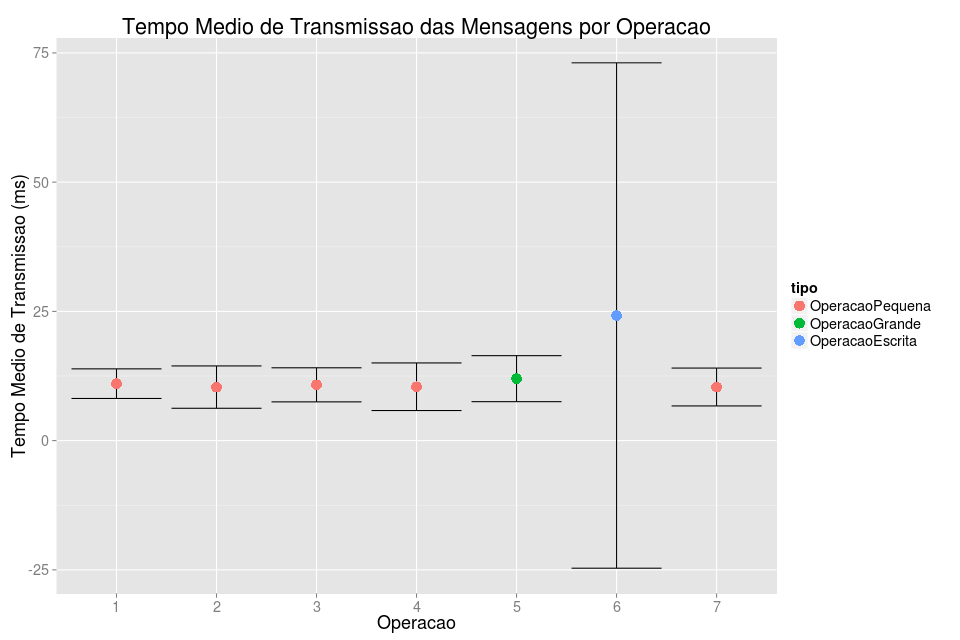
\includegraphics[width=\textwidth]{diagrama/resultadosTempoTransmissao.png}
\caption{Tempo médio, com intervalo de confiança de 95\%, calculado conforme a equação~\ref{eqn:time}, para as sete operações na mesma ordem em que foram descritas, utilizando o protocolo TCP.}
\label{fig:transmissao}
\end{figure}

\subsection{Tamanho de Código}
As operações de redes são, na verdade, parte pequena do código total da aplicação. No servidor, a parte mais extensa do código são claramente as operações de consulta {\it MySQL}. No cliente, além das operações de banco de dados, há dezenas de linhas voltadas apenas para a saída na tela dos {\it prompts} ou a escrita em arquivo.

As operações de redes, mesmo no servidor que faz algumas operações a mais que o cliente, representam muito pouco do código. Considerando-se o servidor, as operações de redes mais os seus testes de erros somam 51 linhas, enquanto o arquivo todo tem 191 (correspondem a cerca de 26\%). Para o cliente, as operações de redes representam 31 de um total de 342 linhas (cerca de 9\%). 

\subsection{Confiabilidade}

Como o protocolo escolhido foi o TCP, que garante confiabilidade na transmissão de mensagens, a confiabilidade esperada era de 100\%. De fato, todas as consultas feitas foram exatamente iguais às geradas localmente para contra-prova, comprovando experimentalmente a confiabilidade do protocolo.

\subsection{Nível de Abstração}

As operações de redes fornecidas pelo sistema são bastante abstratas, apesar de algumas exigirem o entendimento de ponteiros e espaços de memória, meros detalhes da linguagem C. O "diálogo" entre cliente e servidor é resolvido com mensagens, e as operações são tão abstratas quanto imaginamos: baseiam-se em processos de envio ({\it send()} e {\it recv()}). Mesmo operações exclusivas a servidores, como {\it bind()} e {\it listen()}, embora não sejam tão instintivas, uma vez entendido o protocolo, fazem sentido e tem boa abstração. 

Em suma, é possível perceber que toda a complexidade do protocolo está escondida atrás de operações simples.

\section{Conclusões}

No sistema cliente-servidor implementado neste projeto a informação que o servidor retém é a do seu banco de dados e todas as mensagens se baseiam em consultas {\it MySQL}. O tempo total está totalmente influenciado pelo tempo de acesso ao banco, como fica visível na operação de escrita.

Devido a característica desta aplicação apenas uma pequena parte do código do sistema realiza as operações de redes. Apesar disso, essas operações são carregadas pela sua abstração, onde toda a complexidade esta embutida apenas em um comando básico. A abstração condiz com o tempo de execução dessas operações, medidos no tempo de transmissão, que equivale a menos de um quarto do tempo total na maioria das operações.

A confiabilidade garantida pelo protocolo TCP utilizado na comunicação do sistema foi comprovada em todas as consultas. Um futuro trabalho será comparar esses resultados com um sistema que utiliza o protocolo UDP, onde a confiabilidade pode não ser tão perfeita.

\addcontentsline{toc}{section}{\protect\numberline{}Referências}

\singlespace
\bibliographystyle{unsrt}
\bibliography{relatorioUDP}

\end{document}
